% TEXINPUTS=templates/LaTeX2e//: pdflatex paper1_iberamia_timeformer.tex
% TEXINPUTS=templates/LaTeX2e//: bibtex paper1_iberamia_timeformer
% TEXINPUTS=templates/LaTeX2e//: pdflatex paper1_iberamia_timeformer.tex
% TEXINPUTS=templates/LaTeX2e//: pdflatex paper1_iberamia_timeformer.tex
%
% This file is intentionally a planning skeleton, not a full manuscript draft.
\documentclass[runningheads]{llncs}

\usepackage[T1]{fontenc}
\usepackage{graphicx}
\usepackage{amsmath}
\usepackage{amssymb}
\usepackage{booktabs}

\begin{document}

\title{Timeformer: A Controlled Diagnostic Study of Temporal Semantic Traceability}
\titlerunning{Timeformer: Temporal Semantic Traceability}

\author{Anonymous Author}
\authorrunning{Anonymous}

\institute{Institution withheld for review}

\maketitle

\begin{abstract}
Words change meaning over time, yet most computational models treat token
representations as period-independent. We study \emph{temporal traceability}:
whether the same surface token, queried at different periods, occupies
period-appropriate neighborhoods. A model may improve predictive accuracy with
temporal information while still assigning nearly identical neighborhoods across
periods; this gap is our focus.

We introduce Timeformer as a family of token-time conditioning designs. Standard
(no time) and Additive (global time vector) are external baselines. The
Token-Time Transformer, labelled Joint, exposes token identity and period
jointly before self-attention; a Memory-Augmented extension adds causal
prototype memory. All models are trained with masked language modeling on a
synthetic benchmark with known ground-truth trajectories.

The main finding is that token-time conditioning is the effective traceability
mechanism. Joint produces a neighborhood drift of \(-0.614\) for drifting
subjects, versus \(-0.231\) for Standard (stable across seeds).
Probe-based accuracy gains are modest and seed-sensitive, confirming that
geometric diagnostics are more informative than label recoverability. The
Memory-Augmented extension shows no robust improvement; oracle analysis identifies
mean-prototype aggregation as the failure point.

\keywords{Temporal semantics \and Semantic change \and Transformer models \and Traceability \and Diagnostic evaluation}
\end{abstract}

\section{Introduction}
% Target length: 1.0--1.25 pages.
Words do not preserve fixed meanings across time. In 1900, \emph{broadcast}
referred to scattering seeds across a field; today it describes a social media
post reaching millions of users. Most language models, however, take no account
of when a text was written: a word's representation depends on its surrounding
context, but not on the historical period in which it appeared.

The ability to query a word at a specific period matters beyond technical
benchmarks. Whether the shift of \emph{gay} from \emph{cheerful} to its
contemporary sense involved movement toward or away from stigmatized
terms~\cite{hamilton2016diachronic} is an empirical question that requires
\texttt{gay@1920} and \texttt{gay@1980} as directly comparable objects in a
shared space.

The dominant computational approach, lexical semantic change detection (LSCD),
measures such shifts by training distributional representations on time-sliced
corpora and comparing them across
periods~\cite{schlechtweg2020semeval,tahmasebi2021survey}. One model may
associate \emph{broadcast} in 1900 with \emph{sow} and \emph{field}, while
another associates it with \emph{signal} and \emph{audience}; change is inferred
from the distance between the two spaces. It summarizes the shift as a single
similarity score between separately trained models, not as a queryable
\texttt{token@time} object.

A subtler limitation arises when a single model receives temporal information
during training. A model may correctly interpret \emph{virus} as biological
infection in 1900 and as malicious software in 2020, improving word-prediction
accuracy, while still assigning nearly identical neighborhoods across periods.
Prediction accuracy and geometric traceability are separable properties.

We call a representation \emph{temporally traceable} if the same surface token,
queried at different periods, occupies neighborhoods consistent with its meaning
at that period, making \texttt{token@time} a directly inspectable object. This
paper introduces Timeformer as a token-time conditioning family evaluated
against two external baselines: Standard (no time information) and Additive
(global time vector). Joint exposes token identity and period jointly before
self-attention, while a Memory-Augmented extension adds causal prototype memory.
The comparison isolates which form of temporal conditioning produces
traceability in a controlled synthetic benchmark where each subject trajectory
is known.

The paper makes four contributions: it formulates temporal traceability as a
\texttt{token@time} representation problem; identifies token-time conditioning
as the effective mechanism; evaluates traceability with direct subject-level
diagnostics; and shows that mean-pooled historical memory is better understood
as a diagnostic extension than as a robust improvement.


\section{Related Work}
% Target length: under 1 page.
Lexical semantic change detection (LSCD) is the dominant computational framing
for meaning shift. Diachronic word embeddings~\cite{hamilton2016diachronic}
learn one distributional space per time slice, align independently trained
models, and measure movement in neighborhood structure. We share the intuition
that semantic change is geometric, but not the architecture: LSCD yields a
scalar comparison between spaces rather than a jointly parameterized
\texttt{token@time} representation. Standard benchmarks formalize this
task~\cite{schlechtweg2020semeval,tahmasebi2021survey}, while also inheriting
natural-corpus confounds such as frequency and genre drift. Our controlled
benchmark plants trajectories so that traceability can be attributed to model
design rather than corpus composition.

Temporal neural language models avoid separate spaces by conditioning one model
on time. Prior work uses timestamps for knowledge-intensive QA, masked language
modeling, or period-stratified downstream
evaluation~\cite{dhingra2022timeaware,rosin2022timemasking,loureiro2022timelms}. These
results show that temporal conditioning can improve period-appropriate
prediction, but they do not test whether the same token occupies different
neighborhoods at different periods in a shared space. That distinction matters:
accurate time-conditioned predictions may coexist with nearly unchanged
geometry, a dissociation our diagnostics make explicit.

Linear probes provide another partial view. A period probe measures whether time
is recoverable from a hidden state, not whether a token has moved to a different
semantic neighborhood. We therefore report probe accuracy as auxiliary evidence
and treat neighborhood movement as the primary criterion for traceability.

Finally, semantic change may involve bifurcation rather than monotonic drift.
Giulianelli et al.\ show that words can develop coexisting
senses~\cite{giulianelli2020analysing}; mean-pooled representations then collapse
both senses into a centroid that represents neither. Our stable, drifting, and
bifurcating trajectories test this distinction directly, and the memory
extension exposes where mean-pooled prototypes fail.

\section{Controlled Temporal Benchmark}
% Target length: 1.0 page.
The benchmark gives each subject a known temporal trajectory, making it possible
to ask directly whether a model's representation of a subject at \(t0\) has
moved toward the expected neighborhood by \(t9\). This distinguishes it from
natural-language LSCD benchmarks, where ground truth is often annotated or
inferred post-hoc and corpus confounds are hard to separate from genuine semantic
change.

The corpus uses a subject--verb--object (SVO) grammar: every sentence consists
of one subject, one verb, and one object. Two semantic neighborhoods, $N_1$ and $N_2$,
partition the vocabulary of 8 verbs and 8 objects: $N_1$ uses
\(\{V1,\ldots,V4\}\) and \(\{O1,\ldots,O4\}\); $N_2$ uses
\(\{V5,\ldots,V8\}\) and \(\{O5,\ldots,O8\}\). A sentence generated from
$N_1$ therefore looks like \texttt{S5 V2 O3}, while one from $N_2$
looks like \texttt{S5 V6 O8}; the subject token is the same in both cases, but
its co-occurring words differ. Intuitively, the intended meaning of subject
\(s\) at period \(t\) is how often it appears in $N_1$ sentences; formally,
\(P(N_1 \mid s, t)\) is the probability that a sentence is drawn from $N_1$.
The vocabulary contains 30 subjects; each subject's trajectory is determined by
how \(P(N_1 \mid s, t)\) evolves across the 10 periods \(t0\) through \(t9\).

\begin{figure}[t]
\centering
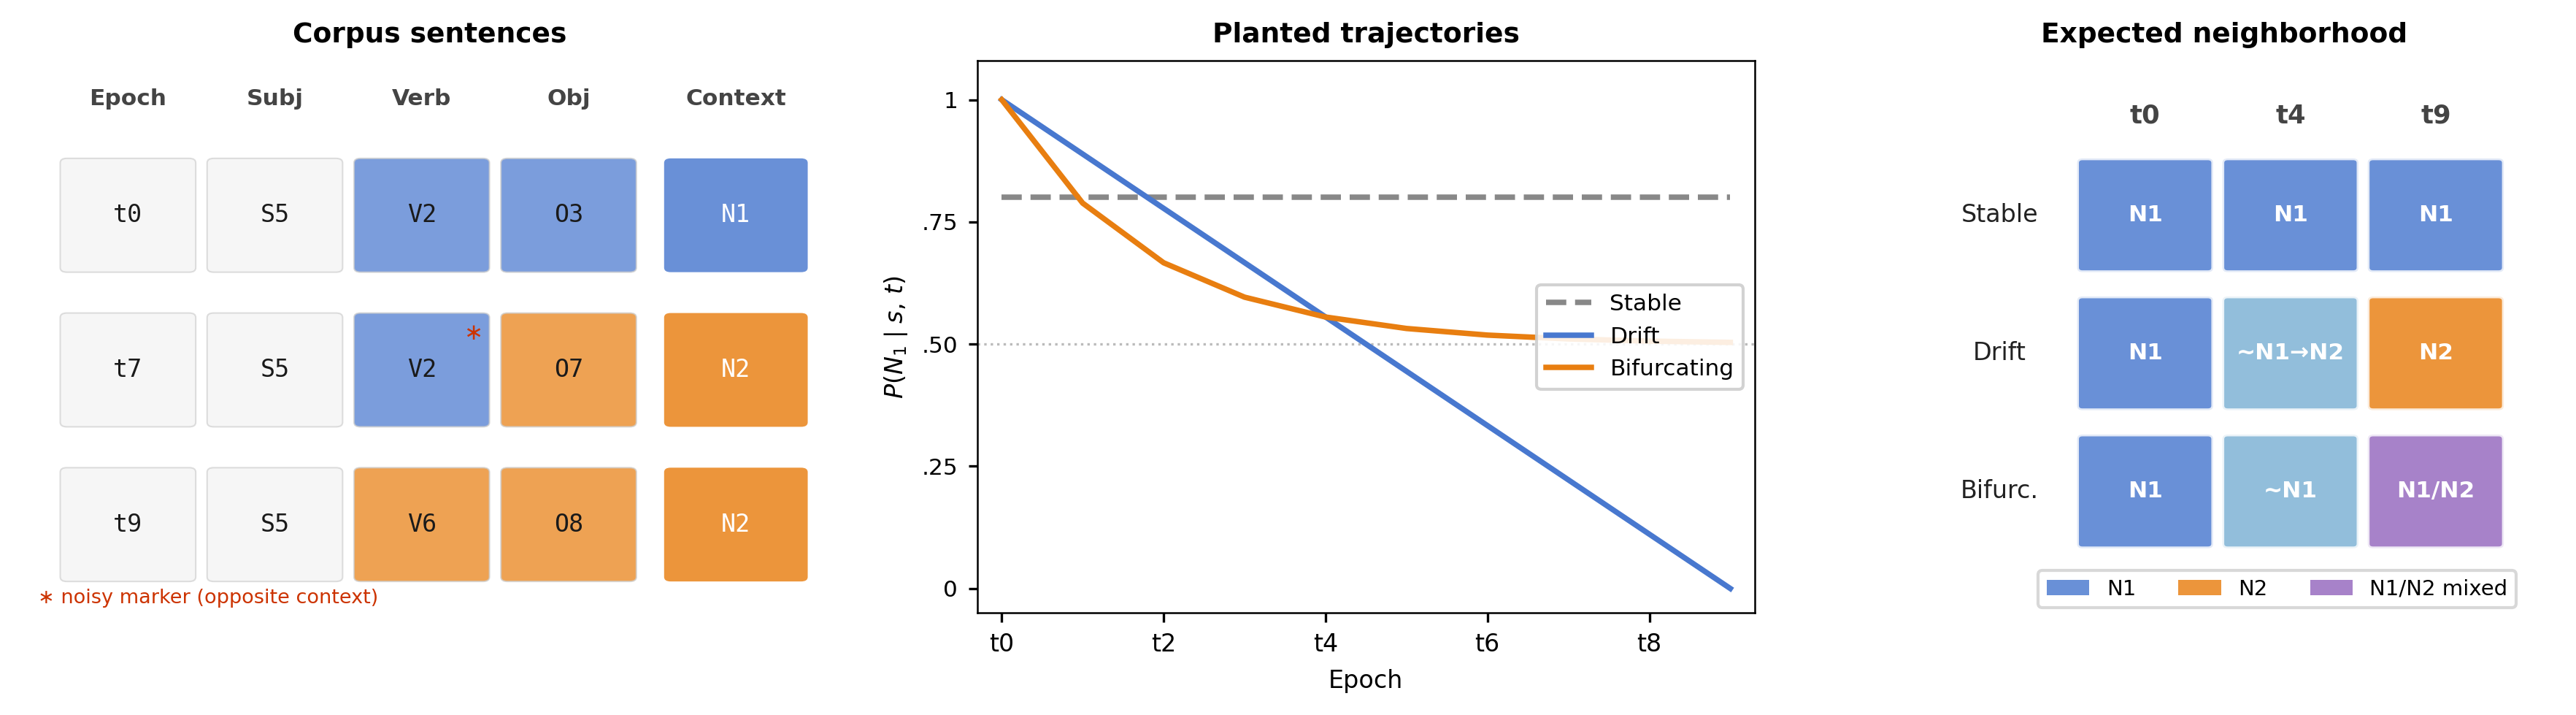
\includegraphics[width=\textwidth]{outputs/figures/figure1_benchmark_design.png}
\caption{Benchmark design overview. \emph{Left}: SVO sentences for a drifting
subject across three periods; an $N_1$ verb appearing in an $N_2$ sentence
at \(t7\) (marked \({\ast}\)) illustrates the deliberate noise in local markers.
\emph{Center}: planted \(P(N_1 \mid s, t)\) trajectories for Stable (flat),
Drift (monotonic), and Bifurcating (levelling at 0.5) subjects across
\(t0\)--\(t9\). \emph{Right}: expected nearest-neighbor behavior for a traceable representation.}
\label{fig:benchmark-design}
\end{figure}

Figure~\ref{fig:benchmark-design} (center) shows the three planted trajectory
classes. Stable subjects maintain an approximately constant \(P(N_1 \mid s, t)\)
throughout. Drift subjects follow a monotonic trajectory from near-exclusive
$N_1$ (\(P(N_1 \mid s, t) \approx 1\) at \(t0\)) to near-exclusive $N_2$
(\(P(N_1 \mid s, t) \approx 0\) at \(t9\)): a drifting subject that appears in
sentences like \texttt{S5 V2 O3} early on will appear in sentences like
\texttt{S5 V6 O8} by the final period. Bifurcating subjects begin in $N_1$
and move toward a mixed state (\(P(N_1 \mid s, t) \approx 0.5\)) where both
neighborhoods appear with equal frequency, approximating two coexisting senses. The
benchmark contains 10 subjects per class.

Each local marker is drawn from the opposite neighborhood 25\% of the time
(Figure~\ref{fig:benchmark-design}, left), so the model cannot recover the
planted neighborhood from co-occurring words alone — it must use subject
identity together with the period. The \texttt{true\_context} label is withheld
from training and used only for evaluation.

The benchmark supports several evaluation conditions. The standard split uses
the same 75\% marker accuracy as training. Two harder splits force the verb, or
both verb and object, to come from the opposite context. An ambiguous split sets
fidelity to 50\%, so local markers carry no reliable signal; only subject
identity and period remain. Two additional conditions test temporal behaviour
directly and are described in Section~5: the contrastive set presents the same
sentence under two different period labels to check whether changing only the
period changes the preferred context; the continuation set uses periods held out from training to test
generalisation. Results throughout are diagnostic evidence in a controlled
setting, not a claim about open-domain historical language.

\section{Timeformer Architecture}
% Target length: 2.0 pages.
Timeformer is designed to make a subject representation depend explicitly on
the queried period. We study this through a controlled comparison: Standard has
no period input, Additive injects a global period vector, Joint exposes token
identity and period jointly before self-attention, and the Memory-Augmented
extension adds causal historical prototypes before the encoder.

All models follow the same outer pipeline. A sentence is tokenized as
\texttt{[CLS] S V O [SEP]}. Each token \(w_i\) is mapped to an input embedding
\(z_i \in \mathbb{R}^d\). The sequence \((z_1,\ldots,z_n)\) is processed by a
Transformer encoder, and the final hidden state at the subject position,
\[
  (h_1,\ldots,h_n) = \mathrm{Encoder}(z_1,\ldots,z_n),
  \qquad h_s = h_{\mathrm{subj}},
\]
is the \texttt{token@time} representation inspected by the diagnostics. All
models are trained with masked language modeling (MLM): some tokens are masked,
and the model must reconstruct them from the remaining tokens and, when
available, the period input. What changes across the design comparison is how
the subject's input embedding \(z_s\) is built before the encoder sees the
sentence.

The temporally informed models use a shared period vector
\(\tau(t) \in \mathbb{R}^d\). It is a learned projection of sinusoidal features
of \(t/T\), where \(T\) is the total number of training periods. In plain terms,
\(\tau(t)\) is the vector representation of the current period. It is distinct
from the position encoding \(p_i\), which only tells the Transformer whether a
token is in subject, verb, or object position. Additive and Joint differ in how
they combine \(\tau(t)\) with token identity; the Memory-Augmented extension
then adds causal memory on top of Joint. Figure~\ref{fig:architecture}
summarizes the comparison.

\begin{figure}[t]
\centering
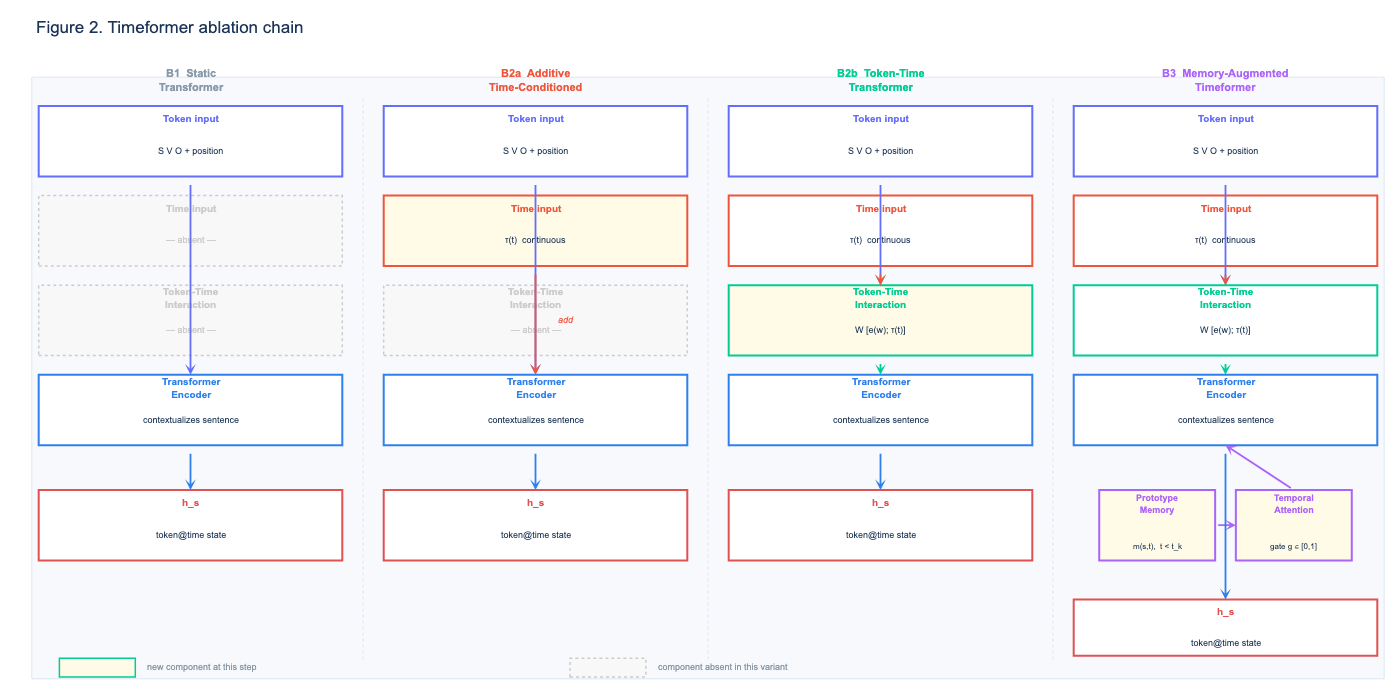
\includegraphics[width=\textwidth]{outputs/figures/figure2_architecture_detail.png}
\caption{Controlled design comparison. \textbf{Standard}: Transformer baseline
with no temporal signal. \textbf{Additive}: temporal baseline that adds the same
period vector to every token. \textbf{Joint}: Token-Time Transformer using joint
token-time projection. \textbf{Memory-Augmented}: extension of Joint with
Prototype Memory and Temporal Attention. New components are highlighted in
yellow; dashed grey boxes mark inactive
components.}
\label{fig:architecture}
\end{figure}

\subsection{Baseline: Standard Transformer}
The Standard baseline asks whether temporal traceability appears without any
period input. Its input embedding is the usual sum of a token embedding and a
position encoding:
\[
  z_i = e(w_i) + p_i .
\]
Because no period signal enters the model, the same sentence at \(t0\) and
\(t9\) produces identical \(h_s\). Standard is the null hypothesis: any
temporal behavior must come only from changes in the observed words.

\subsection{Baseline: Additive Time-Conditioned Transformer}
The Additive baseline asks whether knowing the current period is enough. It
adds the same period vector \(\tau(t)\) to every token:

\[
  z_i = e(w_i) + p_i + \tau(t).
\]

Now \texttt{S5 V2 O3} at \(t0\) and \(t9\) are distinguishable. The subject
embedding is \(e(\texttt{S5})+p_1+\tau(0)\) at \(t0\), and
\(e(\texttt{S5})+p_1+\tau(9)\) at \(t9\). However, the same temporal change is
also applied to the verb and object: \texttt{V2} receives
\(e(\texttt{V2})+p_2+\tau(t)\), and \texttt{O3} receives
\(e(\texttt{O3})+p_3+\tau(t)\). Thus Additive tells the whole sentence which
period it belongs to, but it does not explicitly bind period to each token's
identity. If Additive succeeds, global period information is sufficient. If it
does not, the next question is whether period information must be exposed
jointly with each token before contextualization.

\subsection{Token-Time Transformer}
The Token-Time Transformer, labelled Joint in Figure~\ref{fig:architecture},
asks whether exposing token identity and period jointly before self-attention is
enough. Instead of adding the same period vector to all tokens, Joint
concatenates each token embedding with \(\tau(t)\) and projects the pair:

\[
  z_i = W [e(w_i);\, \tau(t)] + p_i ,
\]

where \(e(w_i), \tau(t) \in \mathbb{R}^d\) and \(W \in \mathbb{R}^{d \times
2d}\). A linear \(W\) does not by itself create nonlinear interaction; rather,
it gives the encoder token-period inputs before self-attention, normalization,
and later nonlinear transformations. For traceability, \texttt{S5} at \(t0\)
and \texttt{S5} at \(t9\) therefore enter the encoder as distinct
period-conditioned inputs, allowing later layers to form token-specific temporal
effects.

\subsection{Memory-Augmented Extension}
The Memory-Augmented extension asks whether causal history helps beyond token-time
conditioning. It starts exactly like Joint: for a current sentence containing
\texttt{S5} at \(t7\), the model first builds token-time input embeddings for
\texttt{[CLS] S5 V O [SEP]}. It then modifies only the subject embedding before
the Transformer encoder sees the sentence.

The additional information comes from Prototype Memory. The extension stores one
prototype vector per subject and past period. A prototype \(m(s,t)\) is the
average representation of subject \(s\) across training sentences from period
\(t\). The memory is causal: at \(t7\), the model may consult
\(\{m(\texttt{S5},0),\ldots,m(\texttt{S5},6)\}\), but not prototypes from
\(t7\) or later.

Temporal attention turns this list of past prototypes into a history summary
for the current subject. Let \(z_s\) be the current Joint subject embedding and
let \(M_s\) be the matrix of available causal prototypes, one row per past
period. The attention operation uses \(z_s\) as the query and \(M_s\) as keys
and values:

\[
  r_s = \mathrm{Attn}(z_s, M_s, M_s).
\]

The vector \(r_s\) summarizes the parts of the subject's history that are most
relevant to the current period. A learned scalar gate \(g\) then decides how
much this history summary should change the current subject embedding:

\[
  \tilde{z}_s =
  z_s + g \cdot
  \left(\mathrm{LN}(z_s + r_s) - z_s\right).
\]

Here, \(\mathrm{LN}\) denotes layer normalization, and \(g\) is a learned
scalar gate initialized at zero so that the extension reduces to Joint at
initialization. Finally, \(\tilde{z}_s\) replaces \(z_s\) in the input
sequence; verb and object embeddings are unchanged, so the subject is the only
token that enters the encoder informed by causal prototype history.

\section{Evaluation Protocol and Diagnostics}
% Target length: 1.25--1.5 pages.
All models in the comparison chain are trained with masked language modeling
over the synthetic SVO corpus. The planted \texttt{true\_context} label is
withheld from training and used exclusively for post-hoc evaluation: it tests
whether the learned subject representation reflects the planted temporal
trajectory. The primary evaluation target is \(h_s\), the final hidden state
at the subject position, because subjects are the lexical items whose meanings
are designed to drift, remain stable, or bifurcate over time.

We use four diagnostics, each targeting a distinct aspect of temporal
representation.

\textbf{D1 -- Linear probe.} Asks whether \(h_s\) encodes the planted context
label at all. We train a linear classifier on \(h_s\) from the standard test
split to predict \texttt{true\_context} and evaluate it on each temporal split.
High accuracy indicates that period-appropriate context is linearly separable in
the representation, but does not reveal whether that separation shifts
systematically over time.

\textbf{D2 -- Context drift score.} Asks whether the neighborhood of a subject
shifts in the expected direction across periods. For each period and subject
class, we retrieve the \(k=10\) nearest neighbors of \(h_s\) by cosine
similarity (excluding the query itself) and record the proportion assigned to
$N_1$. For drifting subjects, this proportion should decrease monotonically from
$t0$ to $t7$; for stable subjects it should remain near its initial value; for
bifurcating subjects it should decrease less steeply, as the representation
splits between neighborhoods rather than migrating from one to the other.

\textbf{D3 -- Contrastive diagnostic.} Asks whether the period label alone
drives representational change. We present the same sentence with two different
period labels and compute the sign-flip rate: the proportion of pairs for which
swapping the period reverses the nearest-neighbor assignment, from
$N_1$-dominant to $N_2$-dominant or vice versa. A model that ignores the period
input produces a sign-flip rate of zero; a model that responds to it produces a
rate above zero.

\textbf{D4 -- Continuation diagnostic.} Asks whether the learned temporal
mapping generalizes beyond training. We evaluate on held-out periods
\(t8\)--\(t9\), excluded from MLM training. A model that has internalized the
direction of change, rather than memorizing period-specific patterns, should
maintain coherent neighborhood assignments in these unseen periods.

The four diagnostics are interpreted through a fixed comparison chain. Additive
vs.\ Standard isolates the effect of adding any temporal signal. Joint
vs.\ Additive tests whether exposing token identity and period jointly before
self-attention is more effective than applying the period globally as a uniform
shift. Memory-Augmented vs.\ Joint tests the contribution of causal prototype
memory, the mechanism most expected to affect D3 and D4.

For the Memory-Augmented extension, we include three controls. In the
\textit{shuffled-memory} control, each subject receives prototypes drawn from a
different subject, disrupting identity-specific history while preserving the
memory pathway. In the \textit{no-history} control, the memory path is present
but empty. In the \textit{oracle-memory} diagnostic, learned prototypes are
replaced by fixed vectors encoding the true historical \(P(N_1 \mid s,t)\)
trajectory. The extension passes the evaluation criterion if it outperforms both
the Token-Time Transformer and the two controls; the oracle diagnostic then
indicates how much headroom remains relative to a perfect memory signal.

\section{Results}
% Target length: 2.5--3.0 pages.
We report results over three training runs. Unless otherwise noted, values are
means over seeds, with the standard deviation shown in parentheses when space
allows. The main finding is that temporal conditioning produces a much
clearer temporal movement in representation space than the Standard Transformer,
with token-time conditioning giving the strongest drifting-subject transition.
The Memory-Augmented extension is informative as a diagnostic, but it
does not provide a robust improvement over the Token-Time Transformer.

\subsection{Temporal Neighborhood Movement}
% Main claim: temporal conditioning produces stronger neighborhood transitions than Standard.
% Use class-specific curves to avoid claiming stable subjects are perfectly flat.
Figure~\ref{fig:context-drift} and Table~\ref{tab:context-drift} show the
context drift score across periods. Standard is a sanity check against a
corpus-only explanation: its weak movement shows that the benchmark alone does
not induce the stronger trajectories observed when period information is
available. For drifting subjects, Standard drops from \(0.618\) to \(0.387\)
(\(\Delta=-0.231\)); Additive reaches \(\Delta=-0.570\); and the Token-Time
Transformer strengthens the transition from \(0.847\) to \(0.233\)
(\(\Delta=-0.614\)). The gap between Joint and Standard is the primary
geometric evidence that token-time conditioning is associated with larger
neighborhood movement for the same subject across periods.

The class-specific curves serve as controls (Table~\ref{tab:context-drift}).
Stable subjects show much smaller movement and no coherent $N_1$-to-$N_2$ trend.
Bifurcating subjects show intermediate drift consistent with a trajectory
toward a mixed state, not a complete transition. The geometric diagnostic
distinguishes all three trajectory classes without relying on probe accuracy
alone.

\begin{figure}[t]
\centering
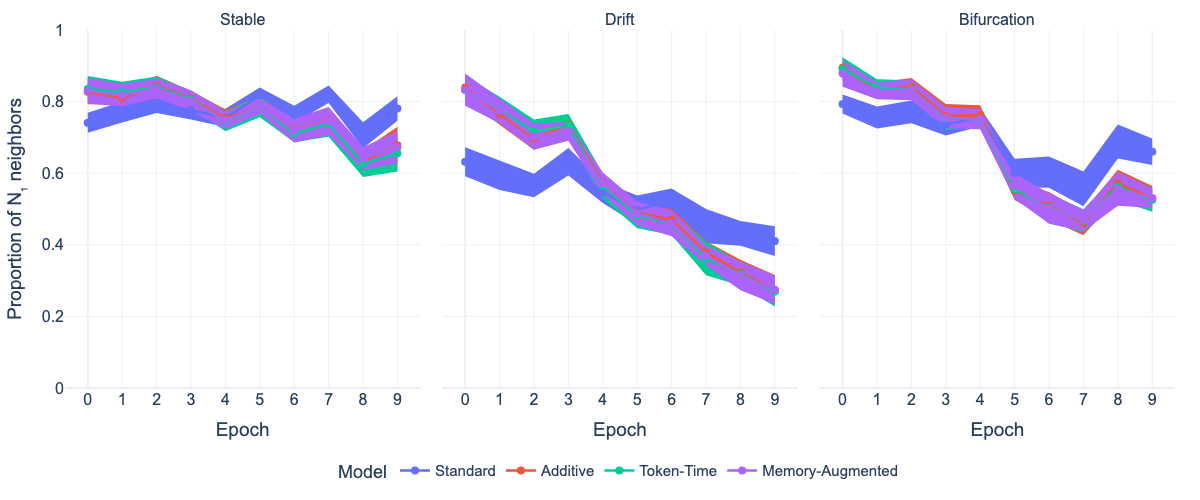
\includegraphics[width=\textwidth]{outputs/figures/figure3_context_drift.png}
\caption{Context drift score across periods. Temporal baselines move drifting
subjects from $N_1$ toward $N_2$ more strongly than the Standard Transformer,
with the Token-Time Transformer showing the largest transition. Stable and
bifurcating subjects provide class-specific controls.}
\label{fig:context-drift}
\end{figure}

\begin{table}[t]
\caption{Context drift score at the first and last periods. Values are
$N_1$ proportions among nearest neighbors; \(\Delta=t9-t0\).}
\label{tab:context-drift}
\centering
\footnotesize
\renewcommand{\arraystretch}{0.88}
\setlength{\tabcolsep}{4pt}
\begin{tabular}{llccc}
\toprule
\textbf{Class} & \textbf{Model} & \textbf{t0} & \textbf{t9} & \(\boldsymbol{\Delta}\) \\
\midrule
Stable & Standard     & 0.736 & 0.756 & +0.020 \\
       & Additive   & 0.790 & 0.658 & -0.132 \\
       & Joint      & 0.843 & 0.641 & -0.203 \\
       & Mem-Aug. & 0.810 & 0.658 & -0.153 \\
\midrule
Drift  & Standard     & 0.618 & 0.387 & -0.231 \\
       & Additive   & 0.847 & 0.278 & -0.570 \\
       & Joint      & 0.847 & 0.233 & -0.614 \\
       & Mem-Aug. & 0.836 & 0.263 & -0.573 \\
\midrule
Bifurcation & Standard     & 0.794 & 0.682 & -0.112 \\
            & Additive   & 0.913 & 0.531 & -0.382 \\
            & Joint      & 0.895 & 0.521 & -0.374 \\
            & Mem-Aug. & 0.905 & 0.517 & -0.388 \\
\bottomrule
\end{tabular}
\end{table}

\subsection{Probe and Contrastive Diagnostics}
The linear probe results show modest accuracy gains that are consistent with,
but weaker evidence for, temporal traceability than the neighborhood analysis.
On the ambiguous split, where local verb and object markers are uninformative,
the Standard Transformer reaches \(0.577\) accuracy, the Additive baseline
reaches \(0.573\), and the Token-Time Transformer reaches \(0.599\). The
corresponding mean delta for token-time conditioning is \(+0.026\), but it is
seed-sensitive: the three runs give \(+0.053\), \(+0.005\), and \(+0.021\).
Probe accuracy alone is insufficient to establish temporal traceability: it
measures recoverability of the planted label, not the geometry of temporal
movement.

The contrastive sign-flip diagnostic gives a different view. The Standard
Transformer has a sign-flip rate of \(0.000\), as expected. The Additive
baseline averages \(0.690\) while the Token-Time Transformer averages \(0.517\),
a counterintuitive ordering. The decoupling arises because sign-flip counts
threshold crossings in individual contrastive pairs, whereas drift score
measures the full trajectory magnitude. A global additive offset can move
representations substantially and generate many threshold crossings, but it
applies the same period signal to every token. Token-time conditioning produces
a slightly stronger drifting-subject trajectory while making the period signal
token-dependent; it does not necessarily cross the threshold in more individual
contrastive pairs. The sign-flip rate confirms that both time-conditioned models
respond to the period input; the neighborhood trajectory (D2) remains the more
informative measure of how the geometry changes across periods.

\begin{table}[t]
\caption{Main traceability diagnostics. Accuracy columns report linear-probe
accuracy on \(h_s\); flip is contrastive sign-flip rate.}
\label{tab:main-results}
\centering
\footnotesize
\renewcommand{\arraystretch}{0.88}
\setlength{\tabcolsep}{5pt}
\begin{tabular}{lcccc}
\toprule
\textbf{Model} & \textbf{Drift} & \textbf{Flip} & \textbf{Ambig.} & \textbf{Cont.} \\
\midrule
Standard   & -0.231 & 0.000 & 0.577 & 0.719 \\
Additive   & -0.570 & 0.690 & 0.573 & 0.754 \\
Joint      & -0.614 & 0.517 & 0.599 & 0.766 \\
Mem-Aug.   & -0.573 & 0.506 & 0.599 & 0.766 \\
\bottomrule
\end{tabular}
\end{table}

\subsection{Memory Diagnostics}
% Report Timeformer honestly: not a stable improvement over Joint, but diagnostically
% useful. Oracle memory may affect sign flip without solving continuation.
The Memory-Augmented Timeformer does not produce a robust gain over the
Token-Time Transformer. On continuation, both models average \(0.766\), and
the per-seed memory deltas are \(+0.013\), \(+0.005\), and \(-0.018\). The
oracle diagnostic clarifies the failure mode: oracle memory improves contrastive
sign flip (\(0.586\) vs. \(0.448\) for the Token-Time Transformer) but not
continuation (\(0.754\) vs. \(0.762\)). Perfect historical prototypes can affect
contrastive temporal behavior, but do not solve the continuation objective under
the current MLM setup.

\begin{table}[t]
\caption{Memory diagnostics. Continuation (D4) is linear-probe accuracy on
held-out periods \(t8\)--\(t9\); flip is the contrastive sign-flip rate (D3).}
\label{tab:memory-diagnostics}
\centering
\footnotesize
\renewcommand{\arraystretch}{0.88}
\setlength{\tabcolsep}{5pt}
\begin{tabular}{lccp{2.8cm}}
\toprule
\textbf{Model} & \textbf{Cont.} & \textbf{Flip} & \textbf{$\Delta$ vs.\ Joint} \\
\midrule
Joint (reference) & 0.762 & 0.448 & -- \\
Mem-Aug. learned  & 0.775 & 0.448 & +0.013 cont.; +0.000 flip \\
Mem-Aug. oracle   & 0.754 & 0.586 & $-$0.008 cont.; +0.138 flip \\
\bottomrule
\end{tabular}
\end{table}

\section{Discussion and Conclusion}
% Target length: 1.25--1.5 pages.
This paper asked whether a Transformer-style encoder can expose a temporally
traceable representation — one in which the same lexical item, queried at
different periods, occupies neighborhoods that reflect its intended temporal
context. The answer, in the controlled benchmark used here, is conditional:
explicit token-time conditioning is the most effective mechanism. A Standard
encoder shows only weak movement, while temporally conditioned models produce
substantially stronger subject-level trajectories. The Token-Time Transformer
is strongest on the primary geometric diagnostic, with a neighborhood drift for
drifting subjects more than twice that of the Standard baseline
(\(-0.614\) vs.\ \(-0.231\)).

The central methodological lesson is that probe accuracy and neighborhood
geometry measure different things. A model can use period information to improve
predictions without producing a representation in which the same lexical item
occupies meaningfully different neighborhoods at different periods. The
evaluation protocol contributes a method for separating these two properties:
geometric diagnostics are necessary alongside label recoverability, as each
captures a distinct aspect of temporal traceability.

This work explores a family of temporal conditioning designs of increasing
complexity. In this benchmark, the Token-Time Transformer is the most effective
instantiation. Its advantage is interpretable as a consequence of the benchmark:
subjects occupy a fixed position, the vocabulary is small, semantic change is
concentrated in the subject token, and planted drift is clean. Under these
conditions, exposing token identity and period jointly before self-attention
gives later layers a clear target for token-specific temporal effects. Additive
remains competitive and is stronger on contrastive sign flip, suggesting that a
global period offset can move many pairs across a binary boundary even when
Joint better captures aggregate neighborhood movement.

The negative result for the Memory-Augmented extension is specific to
mean-pooled prototypes in this controlled setting and should not be read as a
general verdict on causal memory. The oracle diagnostic confirms this: perfect
historical prototypes improve the contrastive sign-flip rate by \(+0.138\) over
the Token-Time Transformer, showing the memory pathway is useful in principle.
The failure of learned prototypes is a failure of aggregation: for bifurcating
subjects, which develop two coexisting senses in later periods, the mean
prototype is a centroid between two clusters, representing neither well.

Several limitations bound these conclusions. The advantage of Joint over
Additive may depend on controlled positions, small vocabulary, and semantic
change concentrated in a known lexical class; in larger corpora with diffuse
change, less regular syntax, or imbalanced periods, it is not guaranteed. More
generally, the benchmark is synthetic, so results should be read as mechanistic
diagnostics rather than evidence of open-domain diachronic performance. The
evaluation covers 30 subjects over three seeds, enough to establish direction
but not precise effect sizes. The MLM objective optimizes token prediction
rather than trajectory geometry, so traceability emerges as a side effect.
Finally, the diagnostic suite was co-designed with the architecture family,
limiting its role as an independent evaluation for models outside this design
space.

Designing memory mechanisms that preserve the internal structure of historical
representations — rather than collapsing them to a single prototype — is the
most direct next step. Evaluating token-time conditioning on natural corpora with
attested semantic change is the necessary path toward claims beyond this
controlled setting.

\begin{credits}

\subsubsection{\discintname}
% TODO: Replace with the final competing interests statement.
The authors have no competing interests to declare that are relevant to the
content of this article.
\end{credits}

% ---- Bibliography ----
\bibliographystyle{splncs04}
\bibliography{references}

\end{document}
